\documentclass[border=0pt]{standalone}

% ---------------------------------------------------------------------------
% Springer-style modern package set
% ---------------------------------------------------------------------------
\usepackage{amsmath}
\usepackage{amssymb}
\usepackage{graphicx}
\usepackage{booktabs}
\usepackage{microtype}
\usepackage[style=numeric, backend=biber]{biblatex}
\usepackage{tikz}
\usetikzlibrary{calc, arrows.meta}
\usepackage{hyperref}
\usepackage{cleveref}

\begin{document}
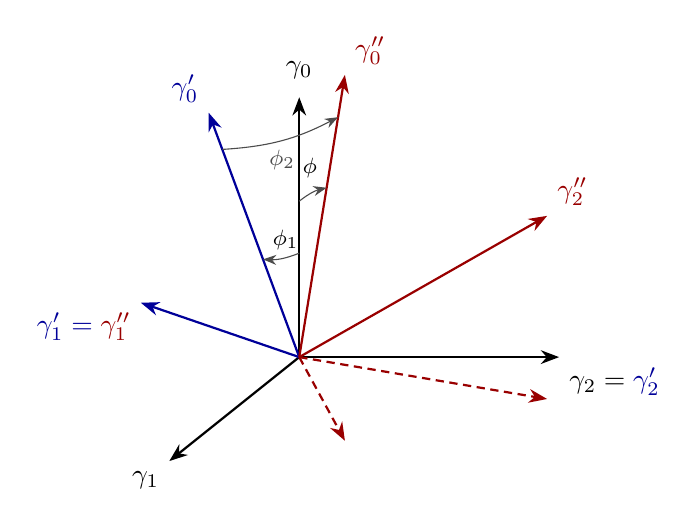
\begin{tikzpicture}[
  >=Stealth,
  scale=2.2,
  x={(-0.5cm,-0.4cm)},
  y={(1.0cm,0.0cm)},
  z={(0.0cm,1.0cm)},
  axis/.style={thick, ->, black},
  axisSp/.style={thick, ->, blue!60!black},
  axisSpp/.style={thick, ->, red!60!black},
  holo/.style={thick, densely dashed, purple!70!black},
  dropLine/.style={thin, densely dashed, black!50},
  projVec/.style={thick, densely dashed, ->, red!60!black}
]

  % Rapidity parameters for consecutive non-collinear boosts
  \def\phione{0.65}
  \def\phitwo{0.55}
  \def\len{1.5}

  % Hyperbolic trigonometric evaluations
  \pgfmathsetmacro{\chA}{cosh(\phione)}
  \pgfmathsetmacro{\shA}{sinh(\phione)}
  \pgfmathsetmacro{\chB}{cosh(\phitwo)}
  \pgfmathsetmacro{\shB}{sinh(\phitwo)}

  \coordinate (O) at (0,0,0);

  % Base frame S (Rest frame)
  \coordinate (g0) at (0, 0, \len);
  \coordinate (g1) at (\len, 0, 0);
  \coordinate (g2) at (0, \len, 0);

  % Singly boosted frame S' (Generator: \gamma_1 \wedge \gamma_0)
  \coordinate (g0p) at ({\len*\shA}, 0, {\len*\chA});
  \coordinate (g1p) at ({\len*\chA}, 0, {\len*\shA});

  % Doubly boosted frame S'' (Generator: \gamma_2' \wedge \gamma_0')
  \coordinate (g0pp) at ({\len*\shA*\chB}, {\len*\shB}, {\len*\chA*\chB});
  \coordinate (g2pp) at ({\len*\shA*\shB}, {\len*\chB}, {\len*\chA*\shB});

  % Projections onto the \gamma_1 \wedge \gamma_2 plane
  \coordinate (g0ppProj) at ({\len*\shA*\chB}, {\len*\shB}, 0);
  \coordinate (g2ppProj) at ({\len*\shA*\shB}, {\len*\chB}, 0);

  % Frame S - Black
  \draw[axis] (O) -- (g1) node[below left] {$\gamma_1$};
  \draw[axis] (O) -- (g2)
    node[below right] {$\gamma_2 = \textcolor{blue!60!black}{\gamma_2'}$};
  \draw[axis] (O) -- (g0) node[above=0.1cm] {$\gamma_0$};

  % Frame S' - Blue
  \draw[axisSp] (O) -- (g1p)
    node[below left] {$\gamma_1' = \textcolor{red!60!black}{\gamma_1''}$};
  \draw[axisSp] (O) -- (g0p) node[above left] {$\gamma_0'$};

  \draw[projVec] (O) -- (g0ppProj) node[below right] {};
  \draw[projVec] (O) -- (g2ppProj) node[right] {};

  % Frame S'' - Red
  \draw[axisSpp] (O) -- (g2pp) node[above right] {$\gamma_2''$};
  \draw[axisSpp] (O) -- (g0pp) node[above right] {$\gamma_0''$};

  % Radial angular arcs staggered to prevent intersection
  \coordinate (ang1_start) at ($(O)!0.40!(g0)$);
  \coordinate (ang1_end) at ($(O)!0.40!(g0p)$);
  \draw[thin, black!70, ->] (ang1_start) to[bend left=12] (ang1_end);
  \node[above right, font=\footnotesize] at (ang1_end) {$\phi_1$};

  \coordinate (angeq_start) at ($(O)!0.6!(g0)$);
  \coordinate (angeq_end) at ($(O)!0.60!(g0pp)$);
  \draw[thin, black!70, ->] (angeq_start) to[bend left=12] (angeq_end);
  \node[above left, font=\footnotesize] at (angeq_end) {$\phi$};

  \coordinate (ang2_start) at ($(O)!0.85!(g0p)$);
  \coordinate (ang2_end) at ($(O)!0.85!(g0pp)$);
  \draw[thin, black!70, ->] (ang2_start) to[bend right=12]
    node[midway, below, font=\footnotesize] {$\phi_2$} (ang2_end);

\end{tikzpicture}
\end{document}
